\section{Experimental results}\sloppy
  \label{sec:exp}

  % Here you evaluate your work using experiments. You start again with a
  % very short summary of the section. The typical structure follows.
  %
  % \mypar{Experimental setup} Specify the platform (processor, frequency, maybe OS, maybe cache sizes)
  % as well as the compiler, version, and flags used. If your work is about performance, 
  % I strongly recommend that you play with optimization flags and consider also icc for additional potential speedup.
  %
  % Then explain what kind of benchmarks you ran. The idea is to give enough information so the experiments are reproducible by somebody else on his or her code.
  % For sorting you would talk about the input sizes. For a tool that performs NUMA optimization, you would specify the programs you ran.

  \mypar{Setup}
  Benchmarks were run on two distinct setups: a node of ETH's Euler cluster, 
  a convential x86 multicore platform, and on ETH's Einstein machine with 
  ssh-access to a Knight's Corner Intel Xeon Phi coprocessor. An Euler node 
  consists of two Intel Xeon E5-2697v2 processors for a total of 24 x86 cores 
  in a dual-socket NUMA setup. The x86 benchmark code was compiled with GCC 
  4.9.2 with OpenMP 4.0, while the Xeon Phi host code was compiled with GCC 
  4.8.2. Both setups used the precompiled version of TBB 4.4 provided by Intel for parallelization.
  \begin{figure}[tb]
    \centering
    \resizebox{\columnwidth}{!}{% File:   buildCompare.tex
% Date:   Mon Jan 18 20:54:14 2016
% Author: Fabian Wermelinger
% Tag:    Buidl comparison
% Copyright 2016 ETH Zurich. All Rights Reserved.
\begin{tikzpicture}[scale=0.7]
  \begin{semilogyaxis}[
    log basis y=10,
    grid=both,
    log ticks with fixed point,
    ymin=0.1,ymax=100,
    xtick={1, 2, 4, 6, 8, 12, 16, 18, 24},
    legend style={legend pos=north east, cells={anchor=west}, 
    font=\footnotesize},
    xlabel={Number of Cores},
    ylabel={Mean Build Time $[s]$}]

    % flann
    \addplot[mark=x, color0, error bars/.cd, y dir=both, y explicit, error bar 
    style={color3}] table[x index=0, y index=1, y error index=2] 
    {./03_results/figs/data_1M/flannBuild.dat};
    \addlegendentry{FLANN}

    % ours
    \addplot[mark=o, color8, error bars/.cd, y dir=both, y explicit, error bar 
    style={color0}] table[x index=0, y index=1, y error index=2] 
    {./03_results/figs/data_1M/randomizedBuild.dat};
    \addlegendentry{Our Implementation}

  \end{semilogyaxis}
\end{tikzpicture}
}
    \caption{Mean build time for the FLANN library and our implementation using 
    $1$~million SIFT vectors.}
    \label{fig:build_comparison}
  \end{figure}
  The Xeon Phi setup additionally uses the MPI library from Intel Parallel 
  Studio XE 2016 when communicating with the Xeon Phi on both host and 
  coprocessor, and the MIC code (\texttt{-mmic}) is compiled using ICC 15.0.0.  
  \begin{figure}[tb]
    \centering
    \resizebox{\columnwidth}{!}{% File:   buildSpeedup.tex
% Date:   Mon Jan 18 22:22:51 2016
% Author: Fabian Wermelinger
% Tag:    Buidl Speedup
% Copyright 2016 ETH Zurich. All Rights Reserved.
\begin{tikzpicture}[scale=0.7]
  \begin{axis}[
    grid=major,
    xtick={1, 2, 4, 6, 8, 12, 16, 18, 24},
    legend style={legend pos=south west, cells={anchor=west}, 
    font=\footnotesize},
    xlabel={Number of Cores},
    ylabel={Speedup Factor}]

    % speedup
    \addplot[mark=x, color8, error bars/.cd, y dir=both, y explicit, error bar 
    style={color0}] table[x index=0, y index=1, y error index=2] 
    {./03_results/figs/data_1M/buildSpeedup.dat};
  \end{axis}
\end{tikzpicture}
}
    \caption{Speedup over the FLANN library for building $4$ randomized k-d 
    trees.}
    \label{fig:build_speedup}
  \end{figure}
  All code was compiled with \texttt{-std=c++11} standard, \texttt{-O3} 
  optimization and \texttt{-march=native} SIMD vectorization (the Euler cluster supports 256-bit vector instructions) for both GCC and 
  ICC. % In particular computing Euclidian distances between high-dimensional input offers a potential gain of vectorization. 

  \mypar{Data set}
  Measurements are done on the TEXMEX~\cite{jegou2011} data set, which is 
  a collection of SIFT~\cite{lowe1999a,lowe2004a} descriptors: 128-dimensional 
  vectors of single precision floating points numbers invariantly describing features in images, commonly used in computer 
  vision to recognize transformations between images taken of the same 
  underlying content. The data set is produced specifically by the authors 
  of~\cite{jegou2011} to test the performance of nearest neighbor algorithms, 
  as it offers a high input size of
  high-dimensional data applied to a common real world problem.
  Comparisons between the vectors are done using the Euclidian distance between them for a relatively low computation intensity of $\approx3/4$ floating point operations per byte. Results presented below are run for the data set containing 1~million reference points queried with 10000 test points for $k=100$.  

  % \mypar{Results}
  % Next divide the experiments into classes, one paragraph for each. In each class of experiments you typically pursue one questions that then is answered by a suitable plot or plots. For example, first you may want to investigate the performance behavior with changing input size, then how your code compares to external benchmarks.
  %
  % For some tips on benchmarking including how to create a decent viewgraph see pages 22--27 in \cite{Pueschel:10}.
  %
  % {\bf Comments:}
  % \begin{itemize}
  %   \item Create very readable, attractive plots (do 1 column, not 2 column plots
  %     for this report) with readable font size. However, the font size should also not be too large; typically it is smaller than the text font size.
  %     An example is in Fig.~\ref{fftperf} (of course you can have a different style).
  %   \item Every plot answers a question. You state this question and extract the
  %     answer from the plot in its discussion.
  %   \item Every plot should be referenced and discussed.
  % \end{itemize}
  %
  % \begin{figure}\centering
  %   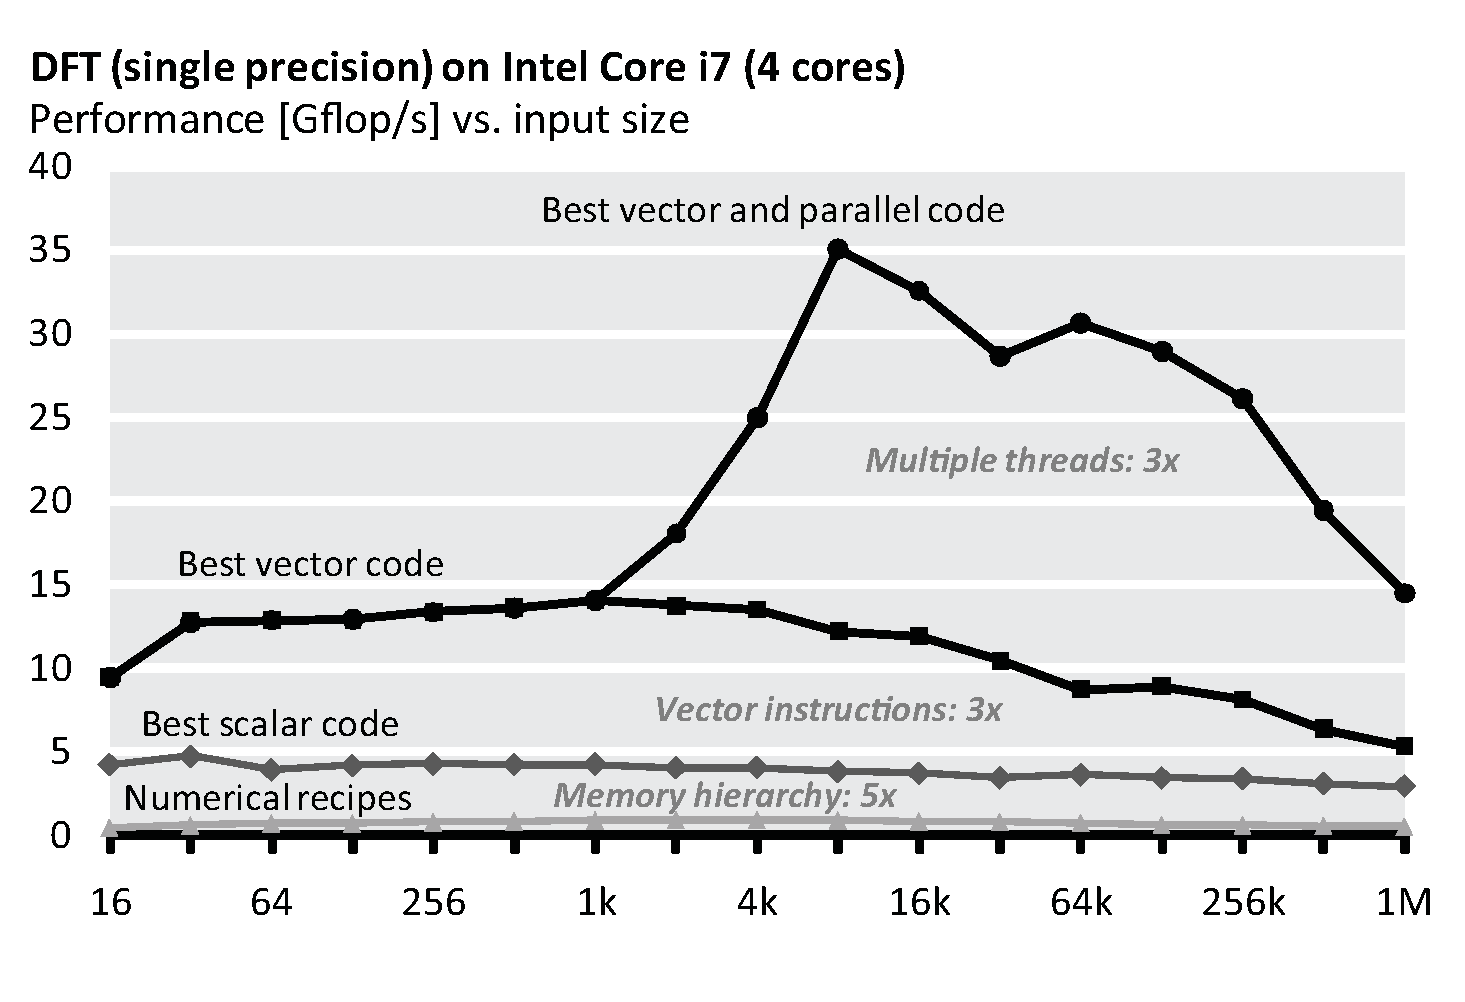
\includegraphics[scale=0.33]{./03_results/figs/dft-performance.eps}
  %   \caption{Performance of four single precision implementations of the
  %   discrete Fourier transform. The operations count is roughly the
  %   same. The labels in this plot are maybe a little bit too small.\label{fftperf}}
  % \end{figure}

  \mypar{Build performance} To evaluate the performance of the build 
  parallelization scheme described in Section~\ref{sec:method}, our 
  implementation is compared to the implementation provided by the FLANN 
  library. Because FLANN implements no parallelization of the tree build, 
  and in particular no trivial parallelization of building $N$ randomized trees in 
  parallel, the implementation described here must scale beyond $N$ processors 
  to demonstrate the advantage of the recursive task
  spawning scheme. In the below we fix $N=4$, as this is enough for satisfactory search performance, while only offering a small initial amount of trivial parallellism up to 4 cores.
  This work contains no demonstration of the suggested 
  parallel build scheme run on Xeon Phi, as compiling the code with ICC for 
  unknown reasons resulted in a build time two orders of magnitude higher than 
  when compiled with GCC, even when run exclusively on the host platform.
  \begin{figure}[tb]
    \centering
    \resizebox{\columnwidth}{!}{% File:   buildCompare.tex
% Date:   Mon Jan 18 20:54:14 2016
% Author: Fabian Wermelinger
% Tag:    Buidl comparison
% Copyright 2016 ETH Zurich. All Rights Reserved.
\begin{tikzpicture}[scale=0.7]
  \begin{semilogyaxis}[
    log basis y=10,
    grid=both,
    log ticks with fixed point,
    xtick={1, 2, 4, 6, 8, 12, 16, 18, 24},
    legend style={legend pos=north east, cells={anchor=west}, 
    font=\footnotesize},
    xlabel={Number of Cores},
    ylabel={Mean Search Time $[s]$}]

    % flann
    \addplot[mark=x, color0, error bars/.cd, y dir=both, y explicit, error bar 
    style={color3}] table[x index=0, y index=1, y error index=2] 
    {./03_results/figs/data_1M/flannSearch.dat};
    \addlegendentry{FLANN}

    % ours
    \addplot[mark=o, color8, error bars/.cd, y dir=both, y explicit, error bar 
    style={color0}] table[x index=0, y index=1, y error index=2] 
    {./03_results/figs/data_1M/randomizedSearch.dat};
    \addlegendentry{Our Implementation}

  \end{semilogyaxis}
\end{tikzpicture}
}
    \caption{Comparison against FLANN for a search of $10000$ query vectors 
    using $4$ randomized k-d trees.}
    \label{fig:search_comparison}
  \end{figure}
  The mean build time of the two implementations are compared 
  in Figure~\ref{fig:build_comparison}, while Figure~\ref{fig:build_speedup} shows the computed speedup over the FLANN 
  library. Because of the lack of parallelization in FLANN, Figure~\ref{fig:build_speedup} can be considered a strong scaling plot with the FLANN single core performance as the baseline. % All measurements shown here are obtained from the Euler compute cluster using one node with $24$ cores.
  The performance is seen to scale well beyond the initial parallel construction of 4 trees, and the build time is down to $0.55$ seconds when utilizing all 24 cores on an Euler node, a speedup of $11$ when compared to the FLANN baseline. This shows a significant benefit of the parallel tree build scheme. As seen for the first data point in Figure~\ref{fig:build_comparison}, the single core performance of FLANN is $45\%$ better than for our implementation, meaning that scalar
  optimizations to our code should have a significant positive impact on the speedup. 

  \mypar{Search performance} Since no novel work is done to improve over the 
  search algorithm implemented for randomized k-d trees in the FLANN library, 
  the performance of the implementation presented here is only expected to 
  match that of FLANN. The contribution of this work is to evaluate the 
  performance of the search algorithm on the Xeon Phi platform.   \begin{figure}[tb]
    \centering
    \resizebox{\columnwidth}{!}{% File:   buildSpeedup.tex
% Date:   Mon Jan 18 22:22:51 2016
% Author: Fabian Wermelinger
% Tag:    Buidl Speedup
% Copyright 2016 ETH Zurich. All Rights Reserved.
\begin{tikzpicture}[scale=0.7]
  \begin{axis}[
    grid=major,
    xtick={1, 2, 4, 6, 8, 12, 16, 18, 24},
    legend style={legend pos=south west, cells={anchor=west}, 
    font=\footnotesize},
    xlabel={Number of Cores},
    ylabel={Speedup Factor}]

    % speedup
    \addplot[mark=x, color8, error bars/.cd, y dir=both, y explicit, error bar 
    style={color0}] table[x index=0, y index=1, y error index=2] 
    {./03_results/figs/data_1M/searchSpeedup.dat};
  \end{axis}
\end{tikzpicture}
}
    \caption{Speedup of $100$-nearest neighbor search against the FLANN library for $10000$ 
    query vectors.}
    \label{fig:search_speedup}
  \end{figure}
  Because of the issues with the build algorithm compiled with ICC as described 
  above, search on the Xeon Phi is done by building the randomized trees on the 
  host processor, then transferring the tree structure using explicit MPI send and receive 
  calls. This allows the host and coprocessor binaries to be built and linked 
  separately with different compilers, relying on Intel's MPI library for 
  interfacing.
  Figure~\ref{fig:search_comparison} shows mean search time observed for a search of $10000$ query vectors using $4$ randomized k-d trees on both the Euler and Xeon Phi platforms, while Figure~\ref{fig:search_speedup} plots the speedup over the FLANN library. % The measurements have been conducted on one node of the Euler platform specified above.  The speedup based on these measurements relative to the FLANN library is shown in Figure~\ref{fig:search_speedup}.
  The scaling between our implementation and that of FLANN is seen in Figure~\ref{fig:search_speedup} to be very similar, but the performance on the Euler node is consistently a factor $0.4$-$0.6$ slower. As with the results for the parallel build described above, this means that our single core performance is lacking when compared to the FLANN library. Because the search parallelizes trivially, the data points in Figure~\ref{fig:search_speedup} are approximately measurements of the same
  number, namely the speedup of the single core performance, resulting in a large propagated error relative to the scale of the plot. The error on the measurements for 12 and 24 cores are considerably lower than the other data points, suggesting that the large deviation is due to jobs contesting resources when running on the Euler batch system and reserving less than the number of cores available on one or two full NUMA nodes.
  For the Xeon Phi the search is run on 240 threads, utilizing the 4 hyperthreads on each of the 60 available cores. The time to solution intersects that of the Euler node at around 12 cores, corresponding to a relative factor of $0.2$ performance per Xeon Phi core to Xeon core. The Xeon Phi numbers do not include the time spent on data transfer, but these numbers become negligible if utilizing the full PCI Express bus for the application described here. When tested for the purpose of this
  work, send/receive calls of MPI only offered $10\%$ of the memory bandwidth promised by PCI Express, while offload mode almost reached the data sheet performance. Even with this performance hit, memory transfers would only add $20\%$ to the total time to solution, down to $2\%$ if the full bandwidth was to be exploited. 

  % mainfile: ./../report.tex
